 \documentclass[c]{beamer}
%\documentclass{beamer}
\listfiles

\mode<presentation>
{
  %\usetheme[deutsch,titlepage0]{KIT}
\usetheme[deutsch]{KIT}
% \usetheme{KIT}

%%  \usefonttheme{structurebold}

  \setbeamercovered{transparent}

  \setbeamertemplate{enumerate items}[circle]
  %\setbeamertemplate{enumerate items}[ball]

}
\usepackage{babel}
\date{}
%\DateText

\newlength{\Ku}
\setlength{\Ku}{1.43375pt}

\usepackage[utf8]{inputenc}
\usepackage[TS1,T1]{fontenc}
\usepackage{array}
\usepackage{multicol}
\usepackage{lipsum}
\usepackage[]{algorithm2e}
\usepackage{amsmath}
\usepackage{color}

\usenavigationsymbols
%\usenavigationsymbols[sfHhdb]
%\usenavigationsymbols[sfhHb]

\subtitle{Algorithmen I SS 14}
\author[]{Lena Winter}

\AuthorTitleSep{\relax}

\institute[ITI]{Institut für Theoretische Informatik}

\TitleImage[width=\titleimagewd]{images/title}

\newlength{\tmplen}

\newcommand{\verysmall}{\fontsize{6pt}{8.6pt}\selectfont}

\title[Algorithmen I SS 14]{Tutorium 9}

\usepackage{alltt}

\TitleImage[width=\titleimagewd]{images/path}

\begin{document}

\begin{frame}
  \maketitle
\end{frame}

\begin{frame}{Minimale Spannbäume}
	\begin{description}
		\item[Gegeben:] Ungerichteter Graph mit Knotenmenge $V$, Kantenmenge $E$ und einer Gewichtsfunktion c
		\item[Gesucht:] Baum mit Knotenmenge $V$, Kantenmenge $F$, $F \subseteq E$ mit minimaler $\sum_{{
   e \in T }} c(e)$, der alle Knoten verbindet 
	\end{description}

	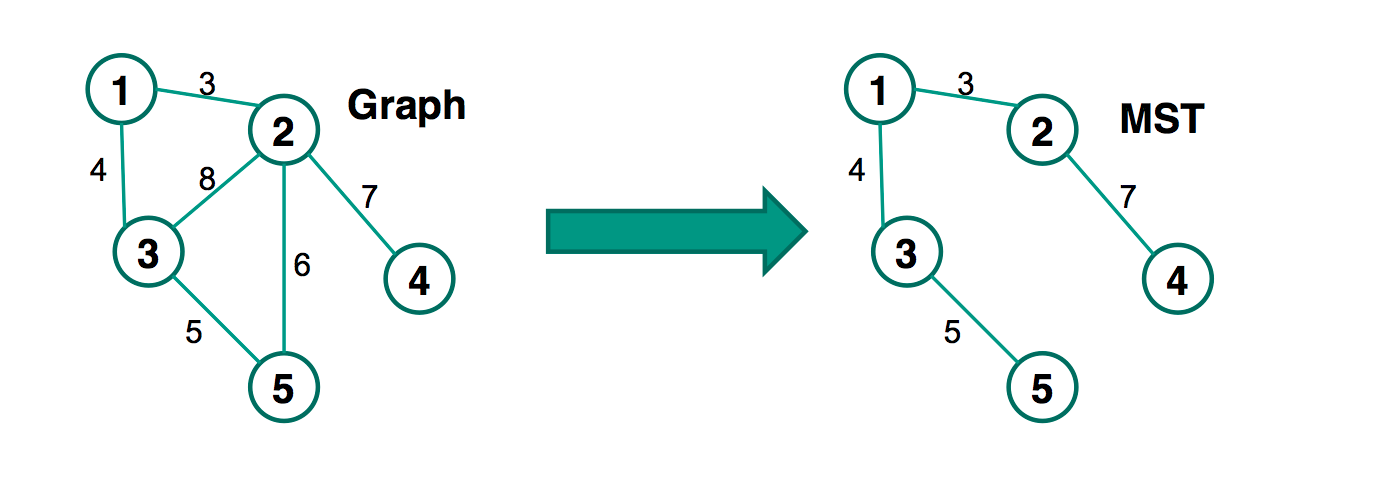
\includegraphics[scale = 0.25]{images/graphs}
\end{frame}

\begin{frame}{Schnitteigenschaft}
	Für eine Beliebige Knotenmenge $S \subseteq V$ gilt für die Kantenmenge C: \\
	\ \\
	\centerline{$C = \{ \{u,v\} \in E: u \in S, v \in V \  \textbackslash \  S \}$}
	\ \\
	\ \\
	$\Rightarrow$ Die Kante mit dem geringsten Gewicht aus $C$ ist Teil des MST
\end{frame}

\begin{frame}{Beispiel}
	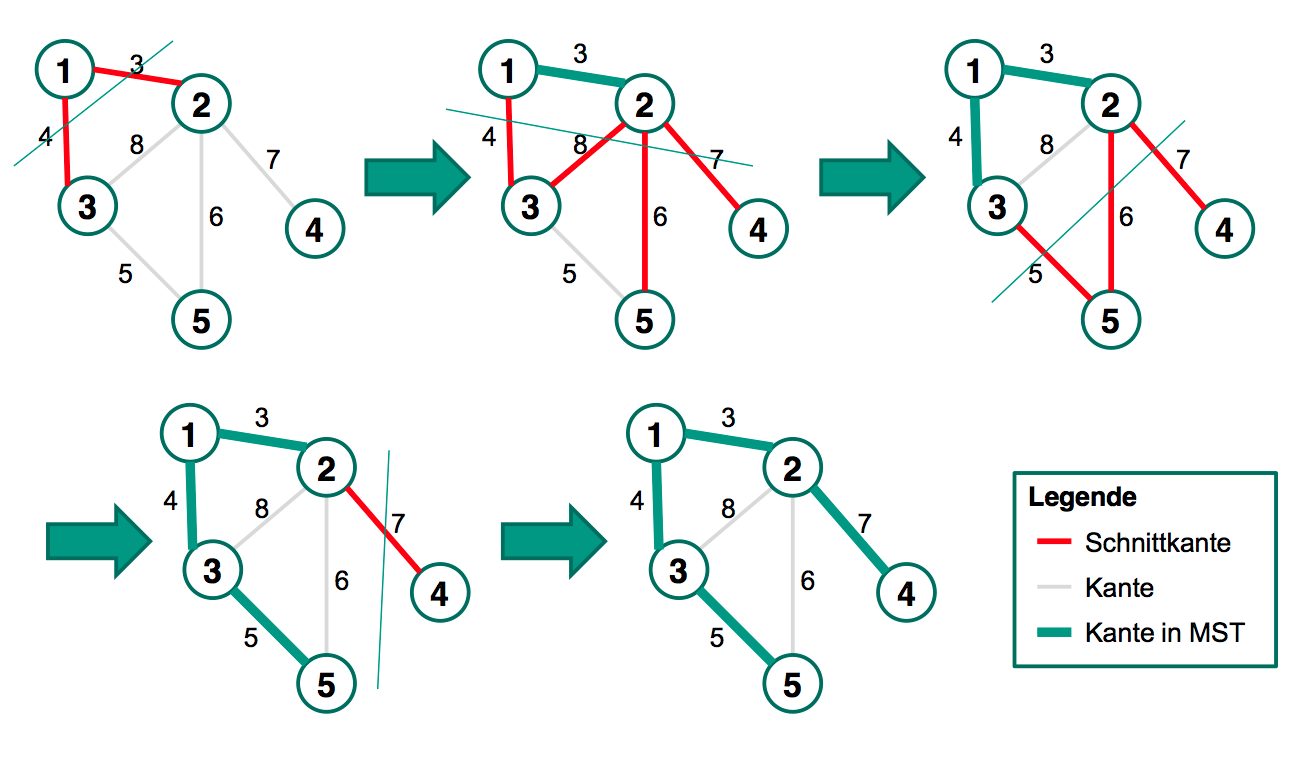
\includegraphics[width=\textwidth]{images/mst}
\end{frame}

\end{document}
